\newpage
\section{Stability Analysis}
\label{sec:stability_analysis}

The imaging algorithms introduced in the previous chapter all rely on a radar system with constant characteristics.
We begin by discussing the physical setup of the experiment, outlining the equipment used and the experimental conditions. 

Additionally, we discuss the preprocessing steps and define the quantities analyzed to assess system stability accurately.
These steps are essential for mitigating noise and ensuring the integrity of the data used for stability analysis.

Furthermore, we explore the concept of self-calibration upon system restart,
investigating how the radar system automatically recalibrates to maintain accuracy and consistency.
Understanding this process is crucial for interpreting stability analysis results accurately and implementing corrective measures effectively.

Finally, we examine the differences between antennas and their impact on radar stability.
Variations in antenna characteristics, such as gain, directivity, and polarization,
can affect signal reception and transmission, influencing the system's overall stability,
and thereby impacting the imaging fidelity.



\subsection{Setup}

The experiment conducted to explore the stability of the sensor consists of setting it up
in a low-reflection environment and placing a corner reflector 
at boresight in front of the sensor at a distance of roughly \SI{1}{\m} (cf. \ref{fig:photo_setup}).

\begin{figure}
    \centering
    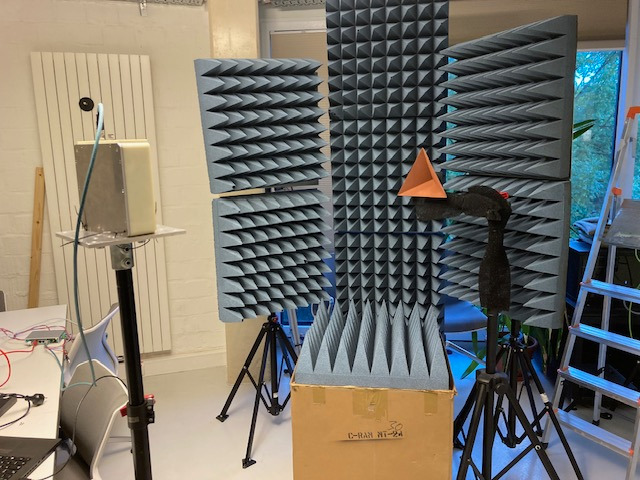
\includegraphics[width=0.6\textwidth]{../figures/aufbau1.jpg}
    \caption{Measurement Setup}
    \label{fig:photo_setup}
\end{figure}

A measurement at relatively short range is preferable because the signal level is higher, 
reducing the impact of noise. The time data collected in all channels is recorded every minute, 
and the temperature readings of the sensor's CPU, FPGA and radar frontend 
are also recorded every minute (cf. \ref{fig:act_temp}).

Due to the static geometry of the setup, the runtime of each transmitted wavefront should be identical.
Thus, the ideal deramped signal should be of a single, constant frequency and without inter-channel phase differences.
For analysis, system runtime and temperature cannot be considered independent variables, as illustrated in \autoref{fig:exp_temp}:
The system starts at ambient temperature, heating up and approaching a stable operating temperature on turning on ($t_0$), and cooling back down after turning off ($t_1$).

\begin{figure}
    \begin{subfigure}[t]{0.45\textwidth}
        \centering
        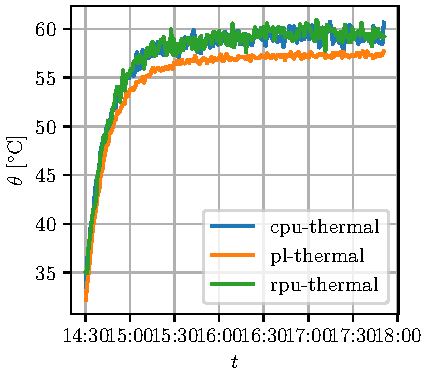
\includegraphics[width=\textwidth]{../figures/actual_temperature.pdf}
        \subcaption{measured temperature}
        \label{fig:act_temp}
    \end{subfigure}
    \begin{subfigure}[t]{0.45\textwidth}
        \centering
        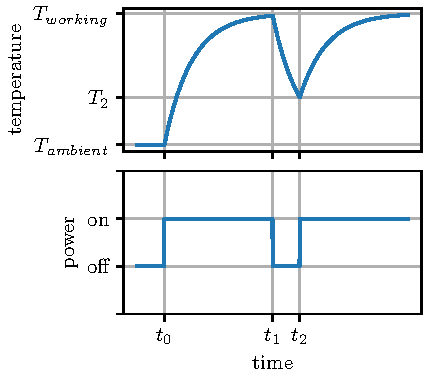
\includegraphics[width=\textwidth]{../figures/expected_temperature.pdf}
        \subcaption{expected temperature}
        \label{fig:exp_temp}
    \end{subfigure}
    \caption{Time Evolution of the Radar System's Temperature}
\end{figure}


In practice, the spectral peak caused by the reflector will also have a certain bandwidth,
and other peaks at higher and lower frequencies will be present due to incomplete shielding and/or unwanted reflections.
Also, the reflector peak may wander if the setup geometry moves.

\subsection{Preprocessing and Analysis}
The primary objective of this experiment is to determine whether the system characteristics remain constant over time. 
This objective can be distilled into an examination of the channel gains $\underline C_k$.
Because of the aforementioned imperfections in the experiment, some preprocessing is required to analize the systematic offsets present in the radar signal.
Multiple additional peaks in the spectrum are visible in \autoref{fig:avg_intensity}.
It is therefore prudent to limit the analysis to only the FFT-bin at the maximum of the peak caused by the reflector.
In theory, this FFT-bin should contain the exact channel gain (see also \autoref{eq:y_fft}):
\begin{align}
    \hat{\underline{C}}_k[l] = \left.\mathcal{F}\{ y_k[m;l]\}\right|_{\Omega=\hat \Omega[l]} \\
    \text{with } \hat\Omega[l] = \arg \underset{subscript}{argument}\max |\mathcal{F}\{ y_k[m;l]\}
\end{align}
In practice, the measurement environment exhibits some minor changes, for example in temperature and humidity, 
which can result in the geometry to shift by up to a few millimeters.
This shows by the spectral maximum shifting over time, as seen in \autoref{fig:refldist}.
\begin{figure}
    \centering
    \begin{subfigure}[t]{.45\textwidth}
        \centering
        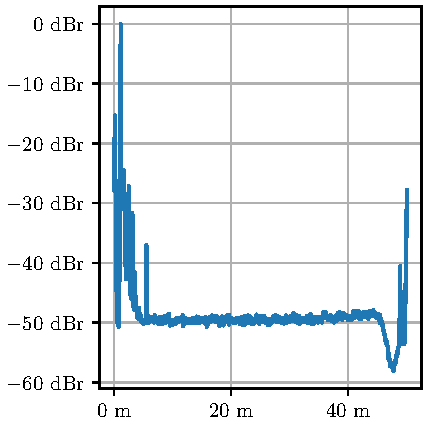
\includegraphics[width=\textwidth]{../figures/interference.pdf}
        \caption{Complete Spectrum}
    \end{subfigure}
    \begin{subfigure}[t]{.45\textwidth}
        \centering
        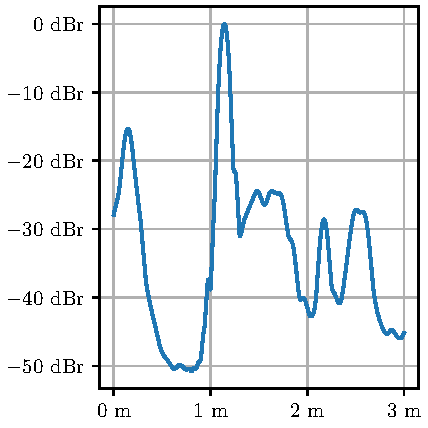
\includegraphics[width=\textwidth]{../figures/interference_zoom.pdf}
        \caption{Zoomed in}
    \end{subfigure}
    \caption{Mean Intensity Spectrum}
    \label{fig:avg_intensity}
\end{figure}
\begin{figure}
    \centering
    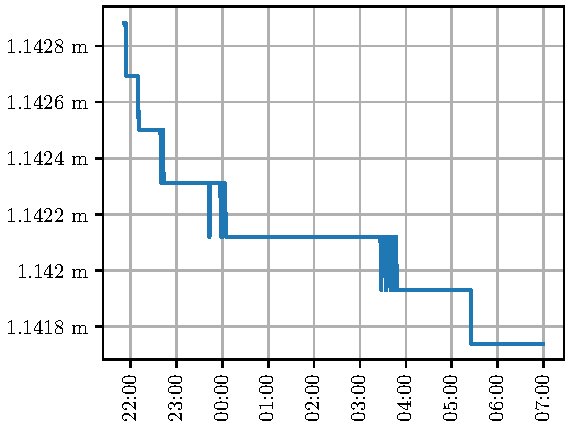
\includegraphics[width=0.6\textwidth]{../figures/refldist.pdf}
    \caption{Change in reflector distance as measured by iMCR}
    \label{fig:refldist}
\end{figure}

The main metric used to assess the stability of the channel gains in the following analysis
will be the complex ratio of the maximum FFT-bin in range to its initial value:
\begin{align}
    \frac{\underline{\hat C}_k[l]}{\underline{\hat C}_k[0]} 
    &= \frac{\mathcal{F}\{y_{k}[m;l]\}(\hat\Omega)}{\mathcal{F}\{y_{k}[m;0]\}(\hat\Omega)} \\
    \text{with } \hat\Omega &= \arg \underset{\Omega}{argument}
\end{align}
Using a logarithmic representation of this ratio,
it can be represented in terms of a level difference in \unit{\dBr} and a phase difference in \unit{\degree}.

\subsection{Effects of System Temperature and Runtime}

Multiple measurements have indicated that, while the amplitude rarely varies by more than \SI{1}{\decibel},
the phase is not as stable over time.
Typically, the mean phase drifts by up to \SI{50}{\degree} in the hours after system startup,
with the rate of change reducing after around four hours.
However, it has to be noted that there is no clear correlation between phase drift and temperature:
the phase continues to drift after the system temperature stabilizes;
the reduction in drift only occurs hours after the system has reached a stable temperature of approximately \SI{60}{\celsius}.

\begin{figure}
    \centering
    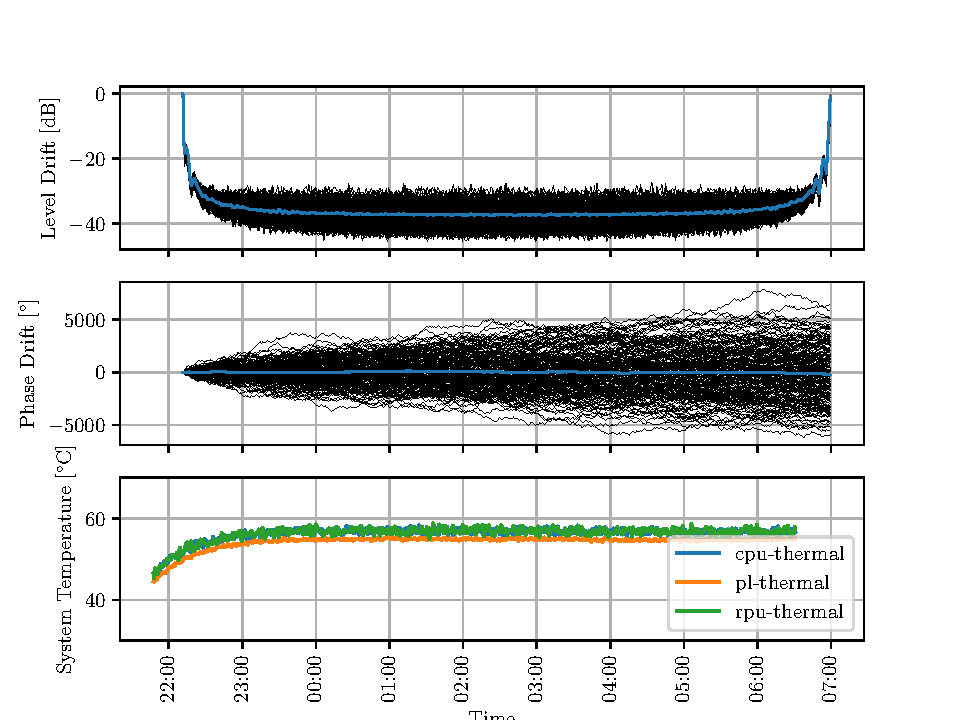
\includegraphics[width=\textwidth]{../figures/meas_24-02-16_phase_drift.pdf}
    \caption{Recorded drift over night}
    \label{fig:weekend}
\end{figure}
TODO : split new measurement into heating up (23:00-8:00) and stable (13:00-12:00).


\subsection{Effects of Self-Calibration}
As described in \autoref{sec:imcr}, the AWR2243P-chips undergo a self-calibration upon initialization.
This initialization can be triggered by either restarting the entire system 
or by re-writing the configuration registers on the radar chips.
Indeed, this initial calibration can be observed in the data (cf. \ref{fig:restart}).
After the connection with the radar has been re-established, the following effects are visible:
\begin{itemize}
    \item slightly increased level: the level in each channel increases by approximately \SI{0.3}{\decibel}
    \item increased incoherence: after the first restart of the system, the drift in both level and phase is distributed more broadly
    \item mean phase: the mean phase drift changes by up to \SI{5}{\degree}
\end{itemize}

\begin{figure}
    \centering
    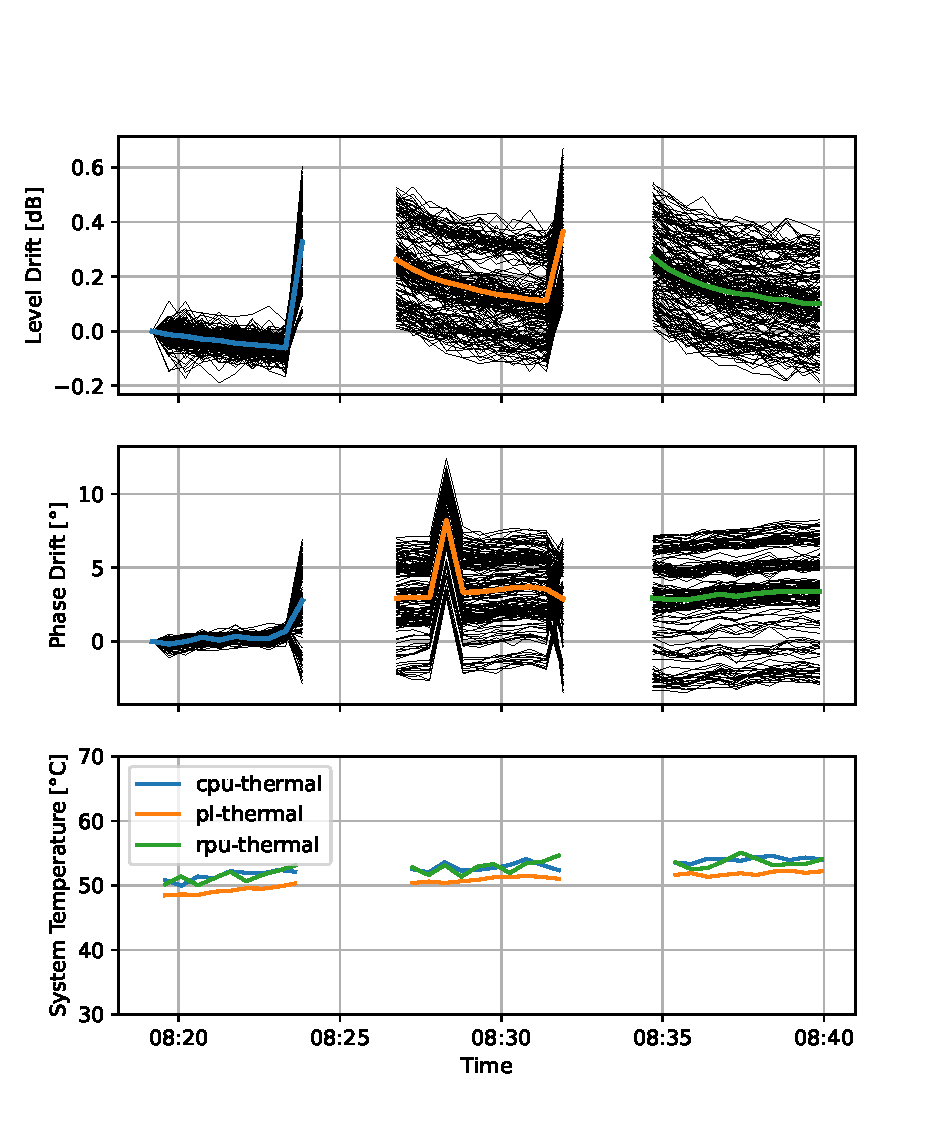
\includegraphics[width=\textwidth]{../figures/meas_23-10-30_reboots_phase_drift.pdf}
    \caption{Recorded drift and temperature with system restart}
    \label{fig:restart}
\end{figure}

TODO: graph jumps to new phase before reboot. confirm or fix.

TODO: quantify amount of discontinuity


\subsection{Antenna Separation}
The channel drifts can be separated into 
\begin{figure}
    \centering
    \includegraphics[options]{../../antenna_drif}
\end{figure}
\subsection{Differences between Antennas}
TODO: Plots, antenna Separation

Comparing the amplitude recorded by all antenna pairs, no channel in particular stands out [PLOT NEEDED].
When looking at the different channels phase drifts, it can be seen that the array becomes less coherent over time.
The distribution of phase shift across channels seems roughly gaussian [PLOT NEEDED], with increasing variance over time.
No antenna pair seems more prone to incoherence than the rest:
across measurements, the maximum outlier (in terms of divergence from the mean phase) cannot be associated with a chip or antenna.

\subsection{Conclusion}
The systematic offsets of the system are now better described.
While the amplitude of the measured signal is relatively stable, the phase is affected more strongly.
All channels' phases drift from both their initial value and each other over time.
It has also be shown that restarting the radar frontend has an effect on the phase, 
since the frontend undergoes an automatic calibration each time.
No clear bias within the array has been found, seeing that across multiple measurements, 
all channels seem to be affected similarly.

Overall, it has been demonstrated that the radar system cannot be considered ideal and
its imaging fidelity will be affected by the growing incoherence during long runtimes.
Furthermore, restarting the system will change the systematic offsets due to the automatic calibration of the radar frontend hardware.
Adaptive online calibration would be required to deal with these effects. \\

To limit the scope of this thesis, the focus is set on the offline-part of the calibration process.
Because the phase and amplitude offsets are affected by the automatic calibration of the system,
this calibration should ideally be repeated on every startup, ideally letting the system temperature stabilize.

An advantage for the offline calibration is that the speed at which the array incoherence grows is limited.
That means that for sufficiently short runtimes, it can be assumed to be static, and therefor, an offline calibration to be sufficient.